\fancychapter{Adaptively Sparse Transformers}
\label{chap:adaptsparse}

\cleardoublepage
\setstretch{1.5}

In the previous chapter, we used transfer learning as a way
to weakly supervise a Transformer model on a low-resource task.
While good results are achieved with this approach, the
architecture of the Transformer is largely uninterpretable,
which can be unappealing if one wishes to understand the
reasons behind the strengths and shortcomings of the model.

To this end, we introduce in the present chapter an approach that
uses \textbf{learnable sparsity} on each of the Transformer's
attention heads. In the context of this thesis, this contribution
leads to neural models that are more \textbf{transparent} in their
decisions. This increased transparency will prove useful in order to
be able to more easily interpret the roles that each attention head
plays in the overall model.

\textit{This chapter is based on \citet{correia2019adaptively}.}

\section{Motivation}

At the heart of the Transformer architecture
(\secref{sec:transformer_bg}) lie \emph{multi-head attention}
mechanisms: each word is represented by multiple different weighted
averages of its relevant context. As suggested by recent works on
interpreting attention head roles, separate attention heads may learn
to look for various relationships between
tokens~\citep{tang2018why,raganato2018analysis,
    marecek-rosa-2018-extracting,bert-rediscovers,specialized}.

The attention distribution of each head in the Transformer is
predicted typically using the \textbf{softmax} normalizing transform.
As a result, all context words have non-zero attention weight. Recent
work on single attention architectures suggest that using sparse
normalizing transforms in attention mechanisms such as sparsemax --
which can yield exactly zero probabilities for irrelevant words --
may improve performance and
interpretability~\citep{malaviya2018sparse,deng2018latent,entmax}.
Qualitative analysis of attention heads
\citep[Figure~5]{vaswani2017attention} suggests that, depending on
what phenomena they capture, heads tend to favor flatter or more
peaked distributions.

\begin{sloppypar}
    Recent works have proposed sparse
    Transformers~\citep{openai_sparse_transf} and adaptive span
    Transformers~\citep{Sukhbaatar2019}. However, the ``sparsity" of those
    models only limits the attention to a contiguous span of past tokens,
    while in this work we propose a \textbf{highly adaptive} Transformer
    model that is capable of attending to a sparse set of words that are
    not necessarily contiguous. \figref{fig:comparison} shows the
    relationship of these methods with ours.
\end{sloppypar}

Our contributions are the following:

\begin{itemize}
    \item We introduce \textbf{sparse attention} into the
          Transformer architecture, showing that it eases
          interpretability and leads to slight accuracy gains.
    \item We propose an adaptive version of sparse attention,
          where the shape of each attention head is {\bf learnable} and can vary continuously and
          dynamically between the dense limit case of \emph{softmax} and the sparse,
          piecewise-linear \emph{sparsemax} case.\footnote{
              Code and pip package available at \url{https://github.com/deep-spin/entmax}.}
    \item We make an extensive analysis of the added interpretability of these
          models, identifying both crisper examples of attention head behavior observed in
          previous work, as well as novel behaviors unraveled thanks to the sparsity
          and adaptivity of our proposed model.
\end{itemize}

\begin{figure}[htbp]
    \centering
    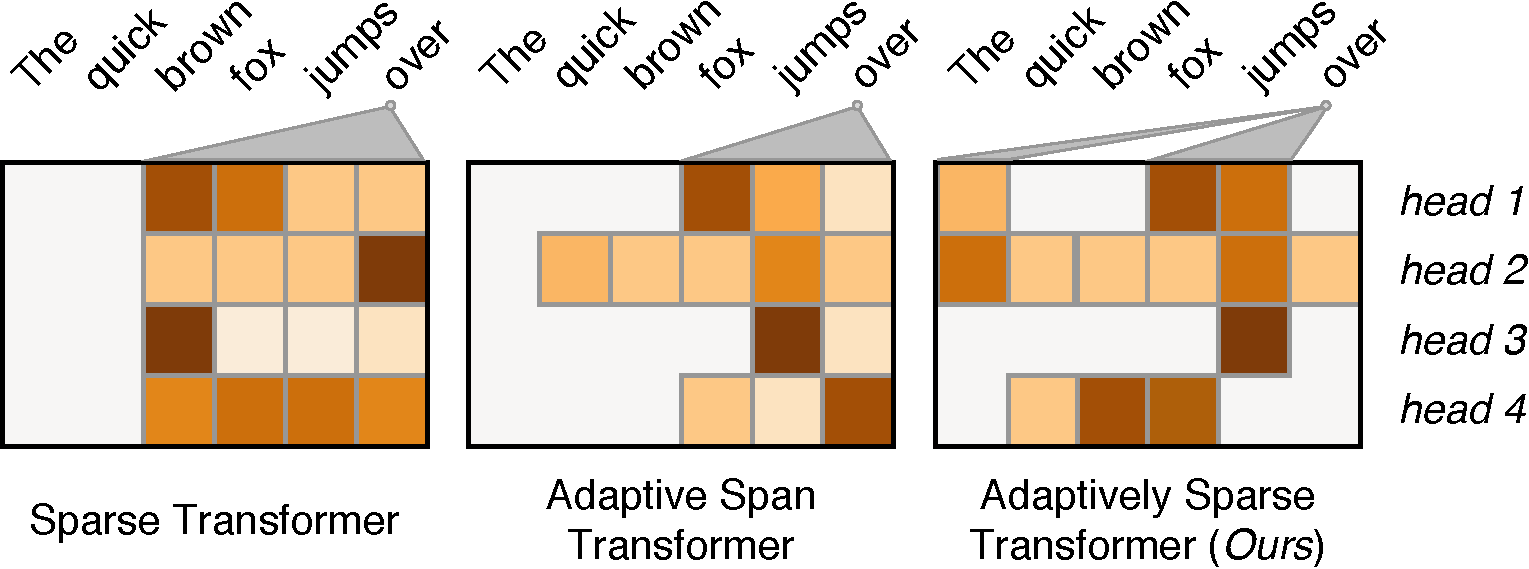
\includegraphics[width=0.95\columnwidth]{Figures/comparison.pdf}
    \caption{Attention distributions of different self-attention heads for the
        time step of the token ``over'', shown to compare our model to other
        related work. While the sparse
        Transformer~\citep{openai_sparse_transf} and the adaptive span
        Transformer~\citep{Sukhbaatar2019} only attend to words within a
        contiguous span of the past tokens, our model is not only able to
        obtain different and not necessarily contiguous sparsity patterns for
        each attention head, but is also able to tune its support over which
        tokens to attend adaptively.}
    \label{fig:comparison}
\end{figure}

\section{Previous Work}

\paragraph*{Sparse attention.}
Prior work has developed sparse attention mechanisms, including
applications to NMT~\citep{sparsemax, malaviya2018sparse, fusedmax,
    shao2019ssn, maruf2019selective}. \citet{entmax} introduced the
\entmaxtext function this work builds upon. In their work, there is a
single attention mechanism which is controlled by a fixed $\alpha$.
In contrast, this is the first work to allow such attention mappings
to \emph{dynamically} adapt their curvature and sparsity, by
automatically adjusting the continuous $\alpha$ parameter. We also
provide the first results using sparse attention in a Transformer
model.

\paragraph*{Fixed sparsity patterns.}
Recent research improves the scalability of Transformer-like networks
through static, fixed sparsity patterns
\citep{openai_sparse_transf,dynamic_conv}. Our adaptively-sparse
Transformer can dynamically select a sparsity pattern that finds
relevant words regardless of their position (\eg,
\figref{fig:head_interro}). Moreover, the two strategies could be
combined. In a concurrent line of research, \citet{Sukhbaatar2019}
propose an adaptive attention span for Transformer language models.
While their work has each head learn a different contiguous span of
context tokens to attend to, our work finds different sparsity
patterns in the same span. Interestingly, some of their findings
mirror ours -- we found that attention heads in the last layers tend
to be denser on average when compared to the ones in the first
layers, while their work has found that lower layers tend to have a
shorter attention span compared to higher layers.

\begin{sloppypar}
    \paragraph*{Transformer interpretability.}
    The original Transformer paper~\citep{vaswani2017attention} shows
    attention visualizations, from which some speculation can be made of
    the roles the several attention heads have.
    \citet{marecek-rosa-2018-extracting} study the syntactic abilities of
    the Transformer self-attention, while \citet{raganato2018analysis}
    extract dependency relations from the attention weights.
    \citet{bert-rediscovers} find that the self-attentions in
    BERT~\citep{devlin2018bert} follow a sequence of processes that
    resembles a classical NLP pipeline. Regarding redundancy of heads,
    \citet{specialized} develop a method that is able to prune heads of
    the multi-head attention module and make an empirical study of the
    role that each head has in self-attention (positional, syntactic and
    rare words). \citet{li2018multi} also aim to reduce head redundancy
    by adding a regularization term to the loss that maximizes head
    disagreement and obtain improved results. While not considering
    Transformer attentions, \citet{jain2019attention} show that
    traditional attention mechanisms do not necessarily improve
    interpretability since softmax attention is vulnerable to an
    adversarial attack leading to wildly different model predictions for
    the same attention weights. Sparse attention may mitigate these
    issues; however, our work focuses mostly on a more mechanical aspect
    of interpretation by analyzing head behavior, rather than on
    explanations for predictions.
\end{sloppypar}

\section{Adaptively Sparse Transformers with \texorpdfstring{{\boldmath $\alpha$}-\entmaxtext}{alpha-entmax}}
\label{sec:adaptive}

We now propose a novel Transformer\footnote{Details on the
    Transformer architecture can be found in
    \secref{sec:transformer_bg}.} architecture wherein we simply replace
softmax with $\alpha$-\entmaxtext{}, described in
\secref{sec:entmax_bg}, in the attention heads. Concretely, we
replace the row normalization $\amap$ in \eqnref{eq:att_scaled_dot}
by

\begin{equation}
    \amap(\bm{Z})_{ij} = \aentmax(\bm{z}_i)_j
\end{equation}

This change leads to sparse attention weights, as long as
$\alpha>1$; in particular, $\alpha=1.5$ is a sensible starting
point~\citep{entmax}.

\paragraph*{Different {\boldmath $\alpha$} per head.}
Unlike LSTM-based seq2seq models, where $\alpha$ can be more easily
tuned by grid search, in a Transformer, there are many attention
heads in multiple layers. Crucial to the power of such models, the
different heads capture different linguistic phenomena, some of them
isolating important words, others spreading out attention across
phrases~\citep[Figure~5]{vaswani2017attention}. This motivates using
different, adaptive $\alpha$ values for each attention head, such
that some heads may learn to be sparser, and others may become closer
to softmax. We propose doing so by treating the $\alpha$ values as
neural network parameters, optimized via stochastic gradients along
with the other weights.

\paragraph*{Derivatives \wrt~{\boldmath $\alpha$}.}
In order to optimize $\alpha$ automatically via gradient methods, we
must compute the Jacobian of the \entmaxtext output \wrt $\alpha$.
Since \entmaxtext is defined through an optimization problem, this is
non-trivial and cannot be simply handled through automatic
differentiation; it falls within the domain of \emph{argmin
    differentiation}, an active research topic in optimization
\citep{gould,optnet}.

One of our key contributions is the derivation of a closed-form
expression for this Jacobian. The next proposition provides
such an expression, enabling \entmaxtext layers with
adaptive $\alpha$. To the best of our knowledge, ours is the first
neural network module that can automatically, continuously vary in
shape away from softmax and toward sparse mappings like sparsemax.

\begin{proposition}\label{prop:grad_alpha}%
    Let $\p^\star \coloneqq \aentmax(\x)$ be the solution of
    \eqnref{eq:define_entmax}.
    Denote the distribution $\tilde{\pp}_i \coloneqq \nicefrac{(\pp_i^\star)^{2 - \alpha}}{
            \sum_j(\pp_j^\star)^{2-\alpha}}$ and let
    $h_i \coloneqq -\pp^\star_i \log \pp^\star_i$.
    The $i$\textsuperscript{th} component of the Jacobian
    $\bm{g} \coloneqq \pfrac{\aentmax(\x)}{\alpha}$ is
    \begin{equation}\label{eq:final_gradient_alpha}
        g_i =%
        \begin{cases}
            \frac{p_i^{\star} - \tilde{\pp}_i}{(\alpha-1)^2} +
            \frac{h_i - \tilde{\pp}_i%
                \sum_j h_j%
            }{\alpha-1},                                                                  & \alpha > 1, \\[1.5ex]
            \frac{h_i \log \pp_i^{\star} - \pp_i^{\star} \sum_j h_j \log p_j^{\star}}{2}, & \alpha = 1.
        \end{cases}
    \end{equation}
\end{proposition}
\noindent%
The proof uses implicit function differentiation and is given in \appref{app:alpha_grad}.

Proposition~\ref{prop:grad_alpha} provides the remaining missing
piece needed for training adaptively sparse Transformers. In the
following section, we evaluate this strategy on neural machine
translation, and analyze the behavior of the learned attention heads.

\section{Experiments}
We apply our adaptively sparse Transformers on four machine translation tasks.
For comparison, a natural baseline is the standard Transformer
architecture using the softmax transform in its multi-head attention mechanisms.
We consider two other model variants in our experiments that make use of different
normalizing transformations:

\begin{itemize}
    \item \textbf{1.5-\entmaxtext:} a Transformer with sparse \entmaxtext
          attention with fixed $\alpha=1.5$ for all heads. This is a novel model,
          since 1.5-\entmaxtext{} had only been proposed for
          RNN-based NMT models~\citep{entmax}, but never
          in Transformers, where attention modules are not just one single
          component of the seq2seq model but rather an integral part of all of
          the model components.%
    \item \textbf{\boldmath $\alpha$-\entmaxtext:} an \textbf{adaptive}
          Transformer with sparse \entmaxtext attention with a different,
          learned $\alpha_{i,j}^t$ for each head.
\end{itemize}

The adaptive model has an additional scalar parameter per attention head per
layer for each of the three attention mechanisms (encoder self-attention,
context attention, and decoder self-attention), \ie,
\begin{equation}
    \big \{ a_{i,j}^{t} \in \reals:~
    i \in \{1, \dots, L\},~
    j \in \{1, \dots, H\},~
    t \in \{\texttt{enc}, \texttt{ctx}, \texttt{dec}\} \big\},
\end{equation}
and we set $\alpha_{i,j}^t = 1 + \sigmoid(a_{i,j}^t) \in ]1, 2[$.
All or some of the $\alpha$ values can be tied if desired, but we
keep them independent for analysis purposes.

\begin{table*}[ht]
    \begin{center}
        \begin{tabular}{lrrrr}
            \toprule
            activation
             & \langp{de}{en} & \langp{ja}{en}
             & \langp{ro}{en} & \langp{en}{de} \\
            \midrule
            $\softmax$
             & 29.79
             & 21.57
             & 32.70
             & 26.02                           \\
            $\aentmax[1.5]$
             & 29.83
             & \textbf{22.13}
             & \textbf{33.10}
             & 25.89                           \\
            $\aentmax[\alpha]$
             & \textbf{29.90}
             & 21.74
             & 32.89
             & \textbf{26.93}                  \\
            \bottomrule
        \end{tabular}
    \end{center}
    \caption{Machine translation tokenized BLEU test results
        on IWSLT 2017 \langp{de}{en},
        KFTT \langp{ja}{en}, WMT 2016 \langp{ro}{en} and
        WMT 2014 \langp{en}{de}, respectively.\label{table:mt}}
\end{table*}

\paragraph*{Datasets.} Our models were trained on 4 machine
translation datasets of different training sizes:

\begin{itemize}[itemsep=.5ex,leftmargin=2ex]
    \item IWSLT 2017 German $\rightarrow$ English
          \citep[\langp{de}{en},][]{cettolooverview}: ~200K sentence pairs.
    \item KFTT Japanese $\rightarrow$ English
          \citep[\langp{ja}{en},][]{neubig11kftt}: ~300K sentence pairs.
    \item WMT 2016 Romanian $\rightarrow$ English
          \citep[\langp{ro}{en},][]{bojar2016findings}: ~600K sentence pairs.
    \item WMT 2014 English $\rightarrow$ German
          \citep[\langp{en}{de},][]{bojar2014findings}: ~4.5M sentence pairs.
\end{itemize}

All of these datasets were preprocessed with byte-pair
encoding~\citep[BPE;][]{sennrich2016neural}, using joint
segmentations of 32k merge operations.

\paragraph*{Training.}
We follow the dimensions of the Transformer-Base model of
\citet{vaswani2017attention}: The number of layers is $L=6$ and
number of heads is $H=8$ in the encoder self-attention, the context
attention, and the decoder self-attention. We use a mini-batch size
of 8192 tokens and warm up the learning rate linearly until 20k
steps, after which it decays according to an inverse square root
schedule. All models were trained until convergence of validation
accuracy, and evaluation was done at each 10k steps for
\langp{ro}{en} and \langp{en}{de} and at each 5k steps for
\langp{de}{en} and \langp{ja}{en}. The end-to-end computational
overhead of our methods, when compared to standard softmax, is
relatively small; in training tokens per second, the models using
$\alpha$-\entmaxtext and $1.5$-\entmaxtext are, respectively, $75\%$
and $90\%$ the speed of the softmax model.

\paragraph*{Results.}
We report test set tokenized BLEU~\citep{papineni2002bleu} results in
\tableref{table:mt}. We can see that replacing softmax by
\entmaxtext{} does not hurt performance in any of the datasets;
indeed, sparse attention Transformers tend to have slightly higher
BLEU, but their sparsity leads to a better potential for analysis. In
the next section, we make use of this potential by exploring the
learned internal mechanics of the self-attention heads.

\section{Analysis}

We conduct high-level analysis of the learned attention heads of the
sparse adaptive Transformer model ($\alpha$-\entmaxtext) trained on
the 4 datasets. We then present, for the higher-resource dataset WMT
2014 English $\rightarrow$ German, a more detailed analysis of the
attention at the individual head behavior. Moreover, we make a
qualitative analysis of the interpretability capabilities of our
models.

\subsection{High-Level Statistics}
\label{sec:stats}

\begin{figure}[ht]
    \centering
    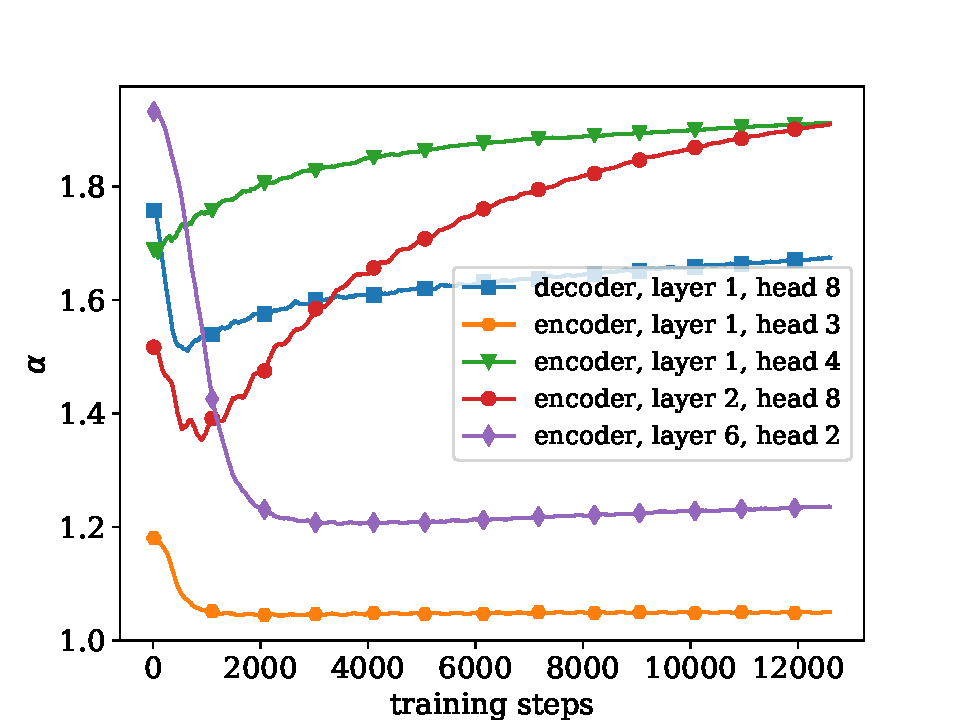
\includegraphics[width=0.85\columnwidth]{Figures/learning_alpha.pdf}
    \caption{\label{fig:learning_alpha}
        Trajectories of $\alpha$ values for a subset of the heads during
        training. Initialized at random, most heads become denser in the
        beginning, before converging. This suggests that dense attention may
        be more beneficial while the network is still uncertain, being
        replaced by sparse attention afterwards.}
\end{figure}

\paragraph*{What kind of {\boldmath $\alpha$} values are learned?}
\figref{fig:learning_alpha} shows the learning trajectories of the
$\alpha$ parameters of a selected subset of heads. We generally
observe a tendency for the randomly-initialized $\alpha$ parameters
to decrease initially, suggesting that softmax-like behavior may be
preferable while the model is still very uncertain. After around one
thousand steps, some heads change direction and become sparser,
perhaps as they become more confident and specialized. This shows
that the initialization of $\alpha$ does not predetermine its
sparsity level or the role the head will have throughout. In
particular, head $8$ in the encoder self-attention layer $2$ first
drops to around $\alpha=1.3$ before becoming one of the sparsest
heads, with $\alpha\approx2$.

The overall distribution of $\alpha$ values at convergence can be
seen in \figref{fig:hist_alphas}. We can observe that the encoder
self-attention blocks learn to concentrate the $\alpha$ values in two
modes: a very sparse one around $\alpha \rightarrow 2$, and a dense
one between softmax and 1.5-\entmaxtext{}. However, the decoder self
and context attention only learn to distribute these parameters in a
single mode. We show next that this is reflected in the average
density of attention weight vectors as well.

\begin{figure}[!htbp]
    \centering
    \begin{subfigure}[b]{.49\linewidth}
        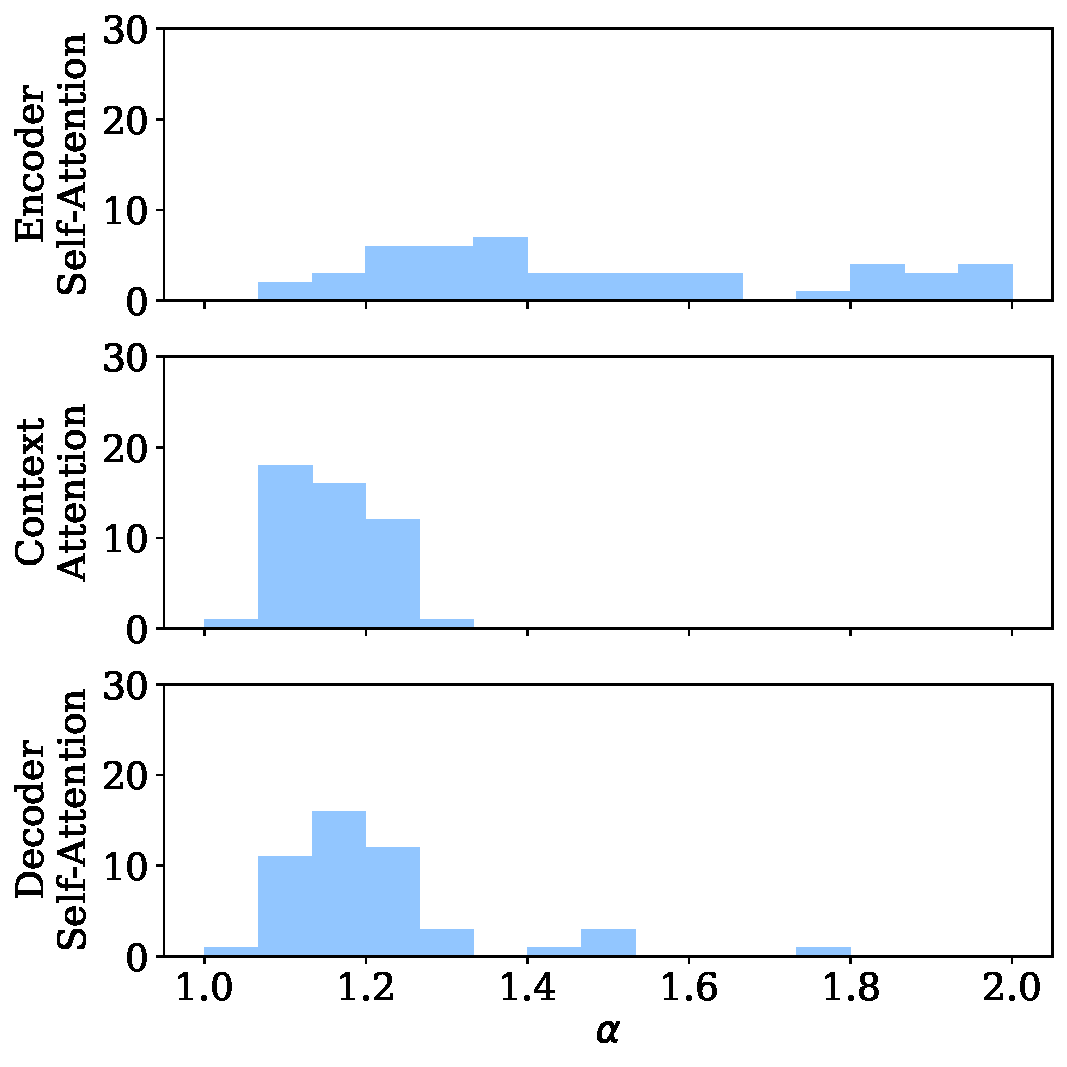
\includegraphics[width=\linewidth]{Figures/hist_alphas_ro.pdf}
        \caption{%
            \label{fig:hist_alphas_ro}%
            WMT 2016 \langp{ro}{en}.}
    \end{subfigure}
    \begin{subfigure}[b]{.49\linewidth}
        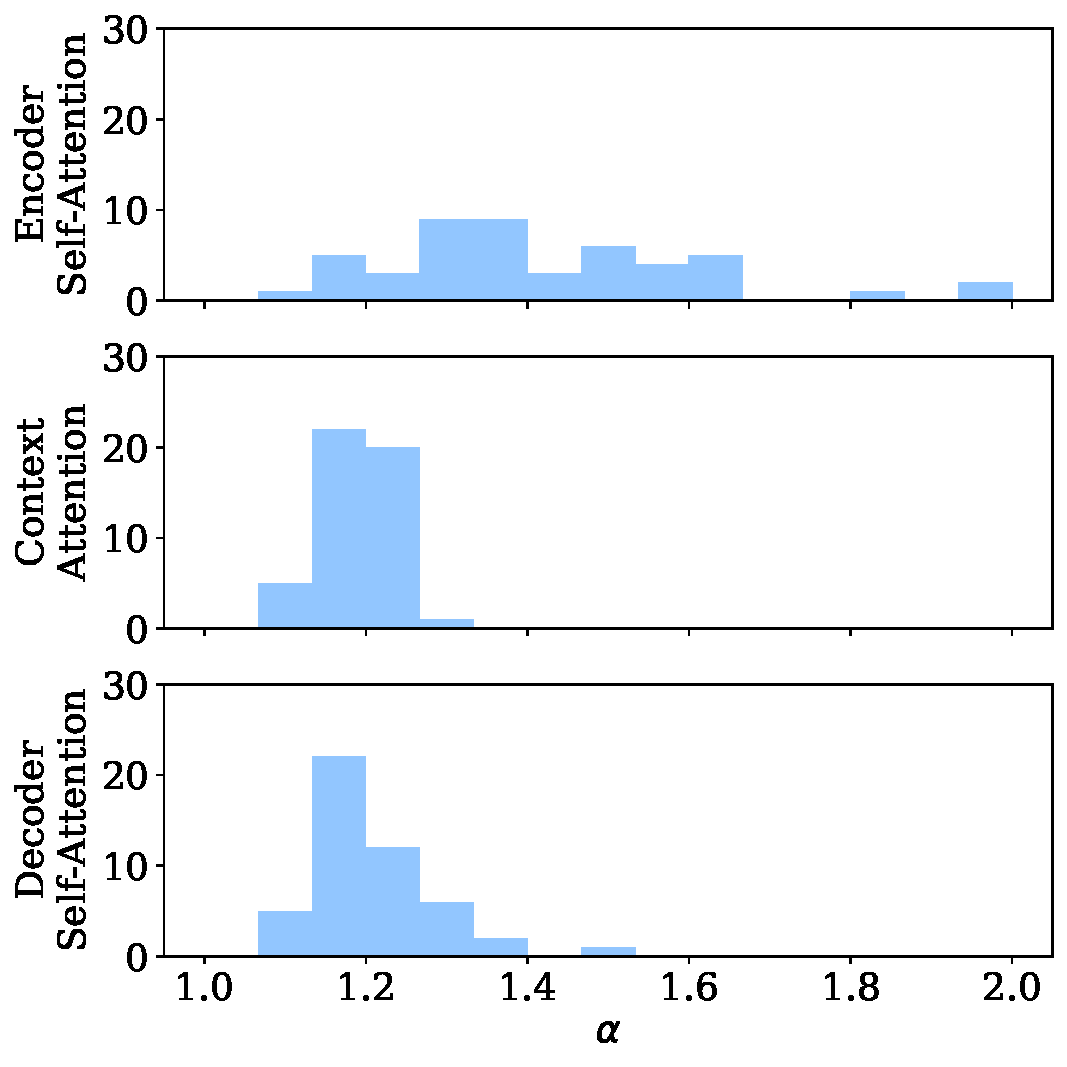
\includegraphics[width=\linewidth]{Figures/hist_alphas_ja.pdf}
        \caption{%
            \label{fig:hist_alphas_ja}%
            KFTT \langp{ja}{en}.}
    \end{subfigure}

    \begin{subfigure}[b]{.49\linewidth}
        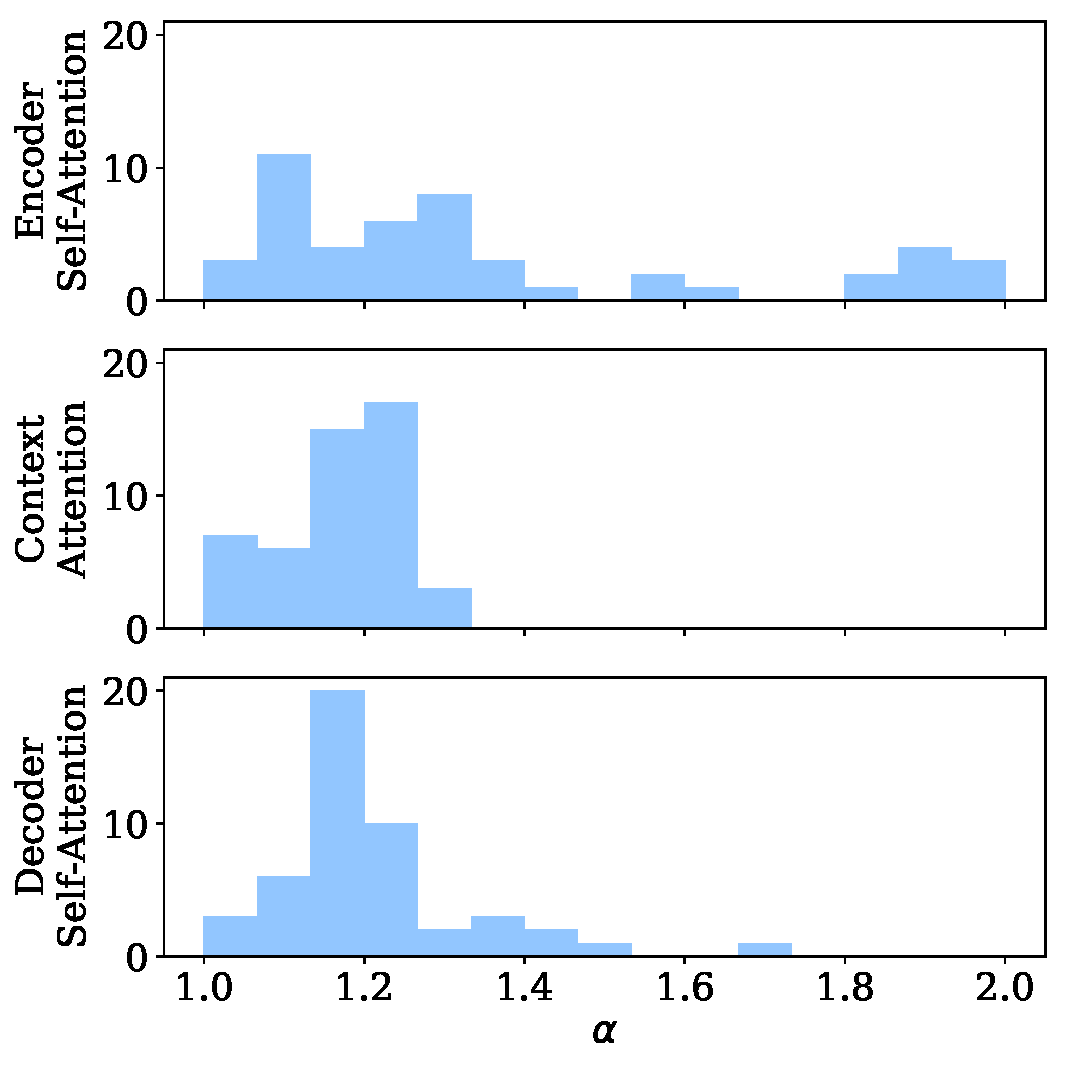
\includegraphics[width=\linewidth]{Figures/hist_alphas.pdf}
        \caption{%
            \label{fig:hist_alphas_en}%
            WMT 2014 \langp{en}{de}.}
    \end{subfigure}
    \begin{subfigure}[b]{.49\linewidth}
        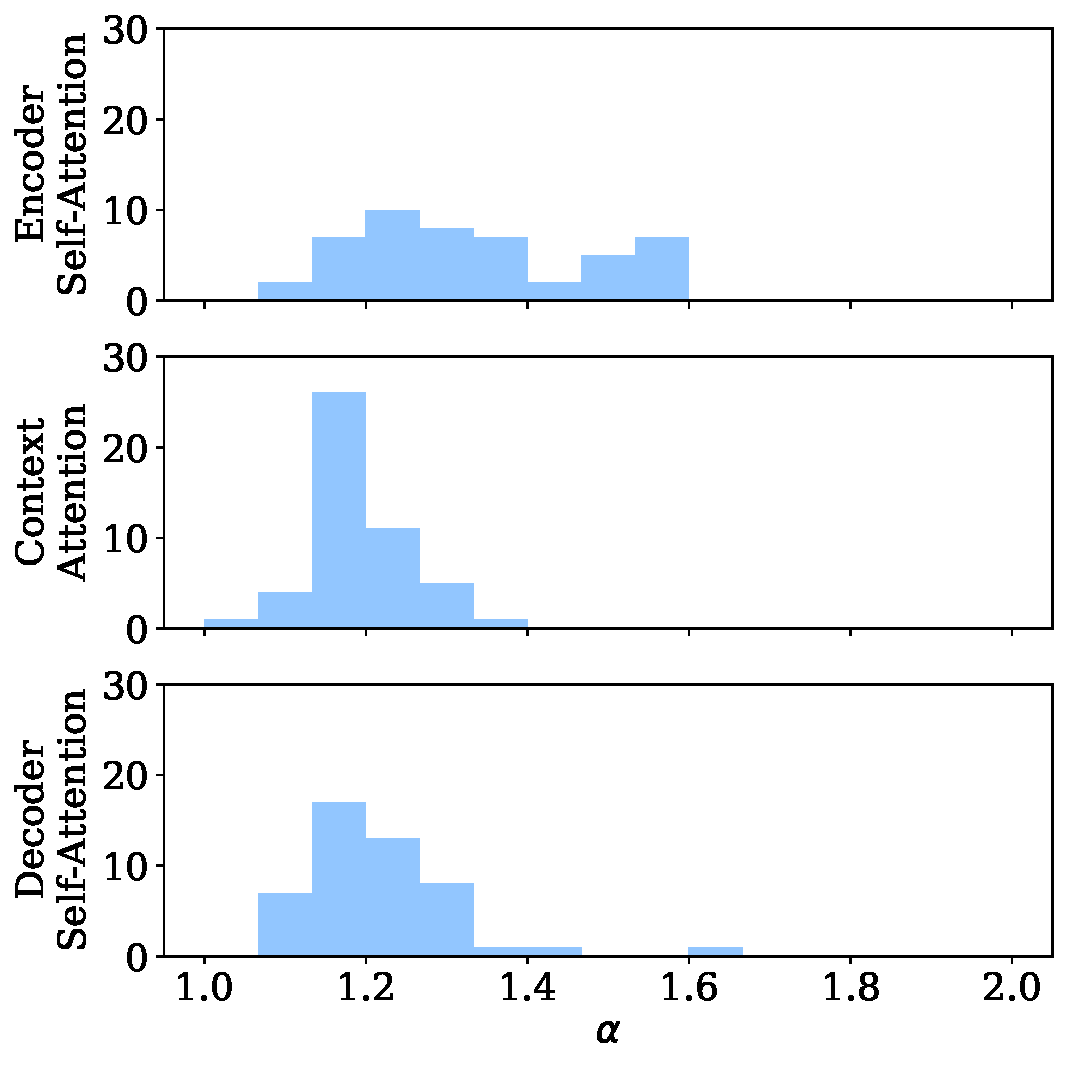
\includegraphics[width=\linewidth]{Figures/hist_alphas_de.pdf}
        \caption{%
            \label{fig:hist_alphas_de}%
            IWSLT 2017 \langp{de}{en}.}
    \end{subfigure}
    \caption{
        Distribution of learned $\alpha$ values per attention block.
        While the encoder self-attention has a bimodal distribution
        of values of $\alpha$,
        the decoder self-attention and context attention have a single mode.}
    \label{fig:hist_alphas}
\end{figure}

\begin{figure}[!htbp]
    \centering
    \begin{subfigure}[b]{.49\linewidth}
        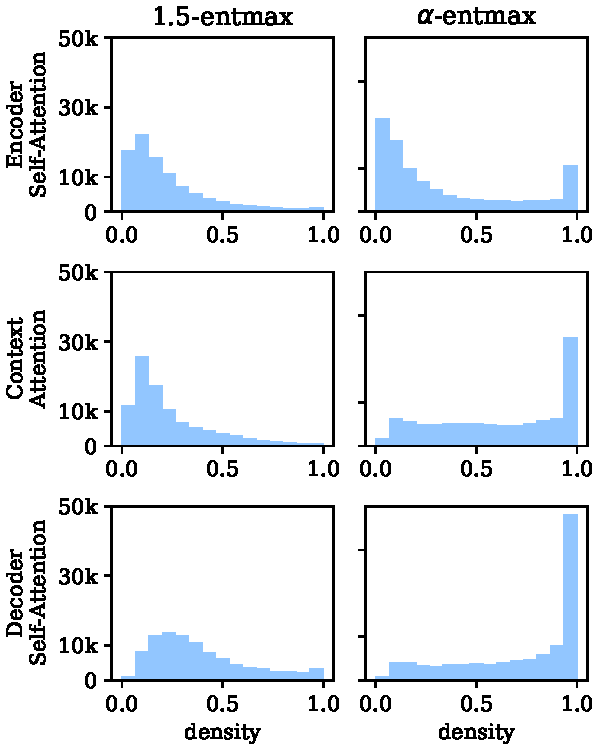
\includegraphics[width=\linewidth]{Figures/hist_densities_ro.pdf}
        \caption{%
            \label{fig:hist_densities_ro}%
            WMT 2016 \langp{ro}{en}.}
    \end{subfigure}
    \begin{subfigure}[b]{.49\linewidth}
        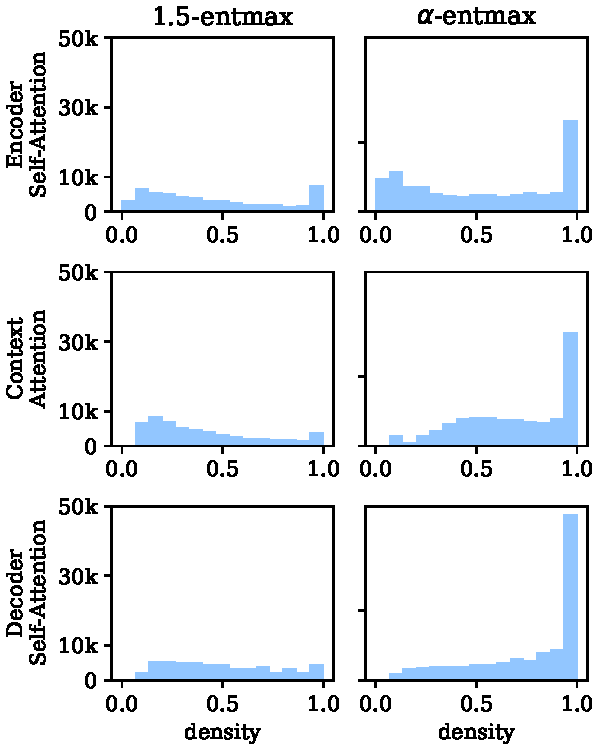
\includegraphics[width=\linewidth]{Figures/hist_densities_ja.pdf}
        \caption{%
            \label{fig:hist_densities_ja}%
            KFTT \langp{ja}{en}.}
    \end{subfigure}

    \begin{subfigure}[b]{.49\linewidth}
        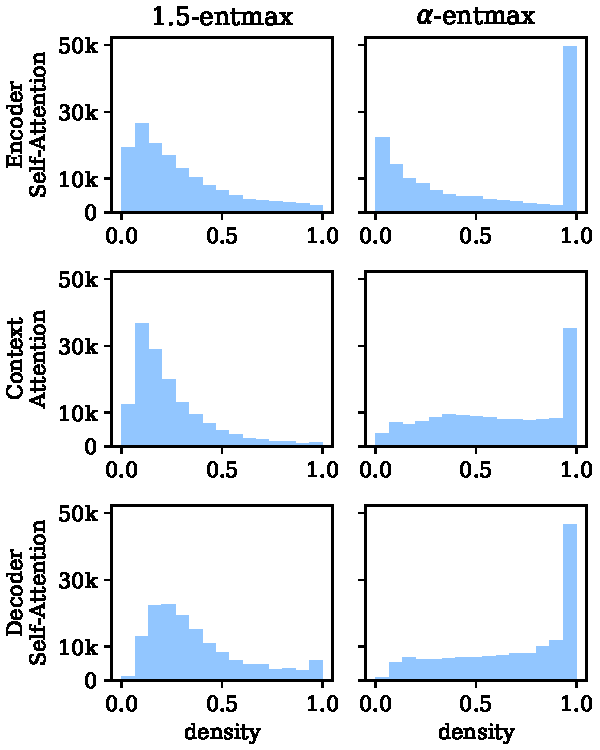
\includegraphics[width=\linewidth]{Figures/hist_densities.pdf}
        \caption{%
            \label{fig:hist_densities_en}%
            WMT 2014 \langp{en}{de}.}
    \end{subfigure}
    \begin{subfigure}[b]{.49\linewidth}
        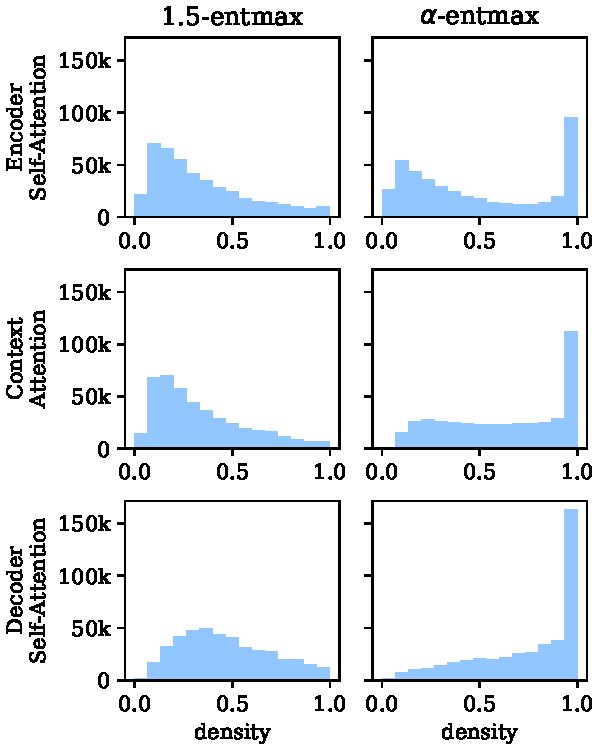
\includegraphics[width=\linewidth]{Figures/hist_densities_de.pdf}
        \caption{%
            \label{fig:hist_densities_de}%
            IWSLT 2017 \langp{de}{en}.}
    \end{subfigure}
    \caption{%
        \label{fig:hist_densities}
        Distribution of attention densities (average number of tokens
        receiving non-zero attention weight) for all attention heads and all
        validation sentences.
        When compared to 1.5-\entmaxtext{}, $\alpha$-\entmaxtext{}
        distributes the sparsity in a more uniform manner, with a clear mode
        at fully dense attentions, corresponding to the heads with low
        $\alpha$. In the softmax case, this distribution would lead to a
        single bar with density 1.}
\end{figure}

\paragraph*{Attention weight density when translating.}
For any $\alpha>1$, it would still be possible for the weight
matrices in \eqnref{eq:head} to learn re-scalings so as to make
attention sparser or denser. To visualize the impact of adaptive
$\alpha$ values, we compare the empirical attention weight density
(the average number of tokens receiving non-zero attention) within
each module, against sparse Transformers with fixed $\alpha=1.5$.

\begin{sloppypar}
    \figref{fig:hist_densities} shows that, with fixed $\alpha=1.5$, heads
    tend to be sparse and similarly-distributed in all three attention
    modules. With learned $\alpha$, there are two notable changes: (i) a
    prominent mode corresponding to fully dense probabilities, showing
    that our models learn to combine sparse and dense attention, and (ii)
    a distinction between the encoder self-attention -- whose background
    distribution tends toward extreme sparsity -- and the other two
    modules, who exhibit more uniform background distributions. This
    suggests that perhaps entirely sparse Transformers are suboptimal.
\end{sloppypar}

The fact that the decoder seems to prefer denser attention
distributions might be attributed to it being auto-regressive, only
having access to past tokens and not the full sentence. We speculate
that it might lose too much information if it assigned weights of
zero to too many tokens in the self-attention, since there are fewer
tokens to attend to in the first place.

Teasing this down into separate layers,
\figref{fig:head_density_per_layer} shows the average (sorted) density of
each head for each layer. We observe that $\alpha$-\entmaxtext{} is
able to learn different sparsity patterns at each layer, leading to
more variance in individual head behavior, to clearly-identified
dense and sparse heads, and overall to different tendencies compared
to the fixed case of $\alpha=1.5$.

\begin{figure}[!htbp]
    \centering
    \begin{subfigure}[b]{.49\linewidth}
        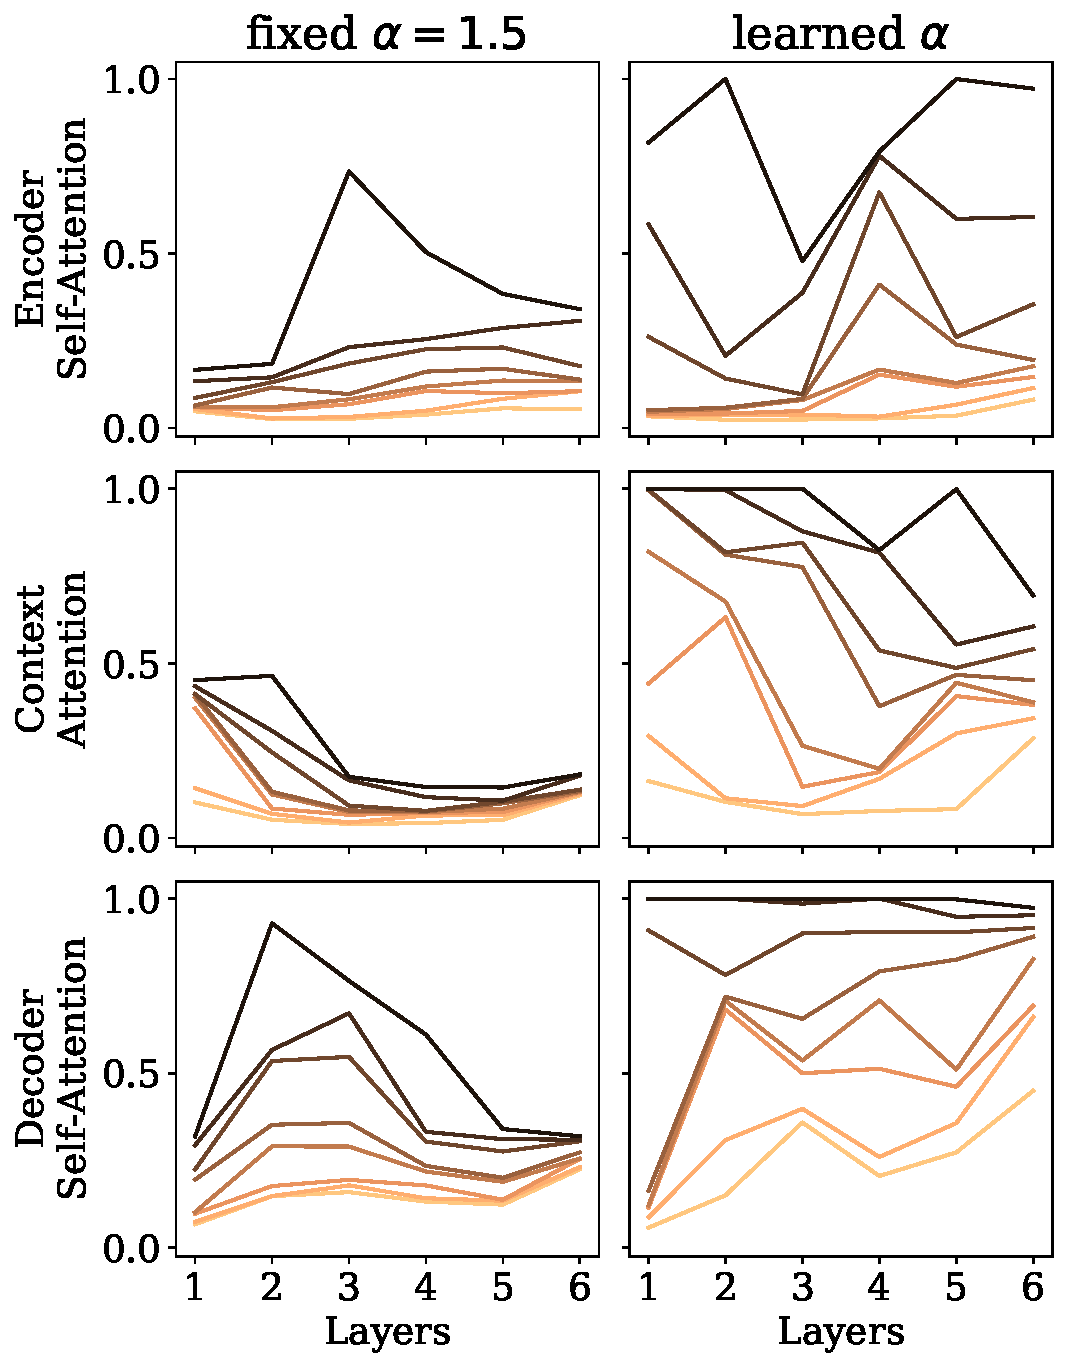
\includegraphics[width=\linewidth]{Figures/head_density_per_layer_ro.pdf}
        \caption{%
            \label{fig:head_density_per_layer_ro}%
            WMT 2016 \langp{ro}{en}.}
    \end{subfigure}
    \begin{subfigure}[b]{.49\linewidth}
        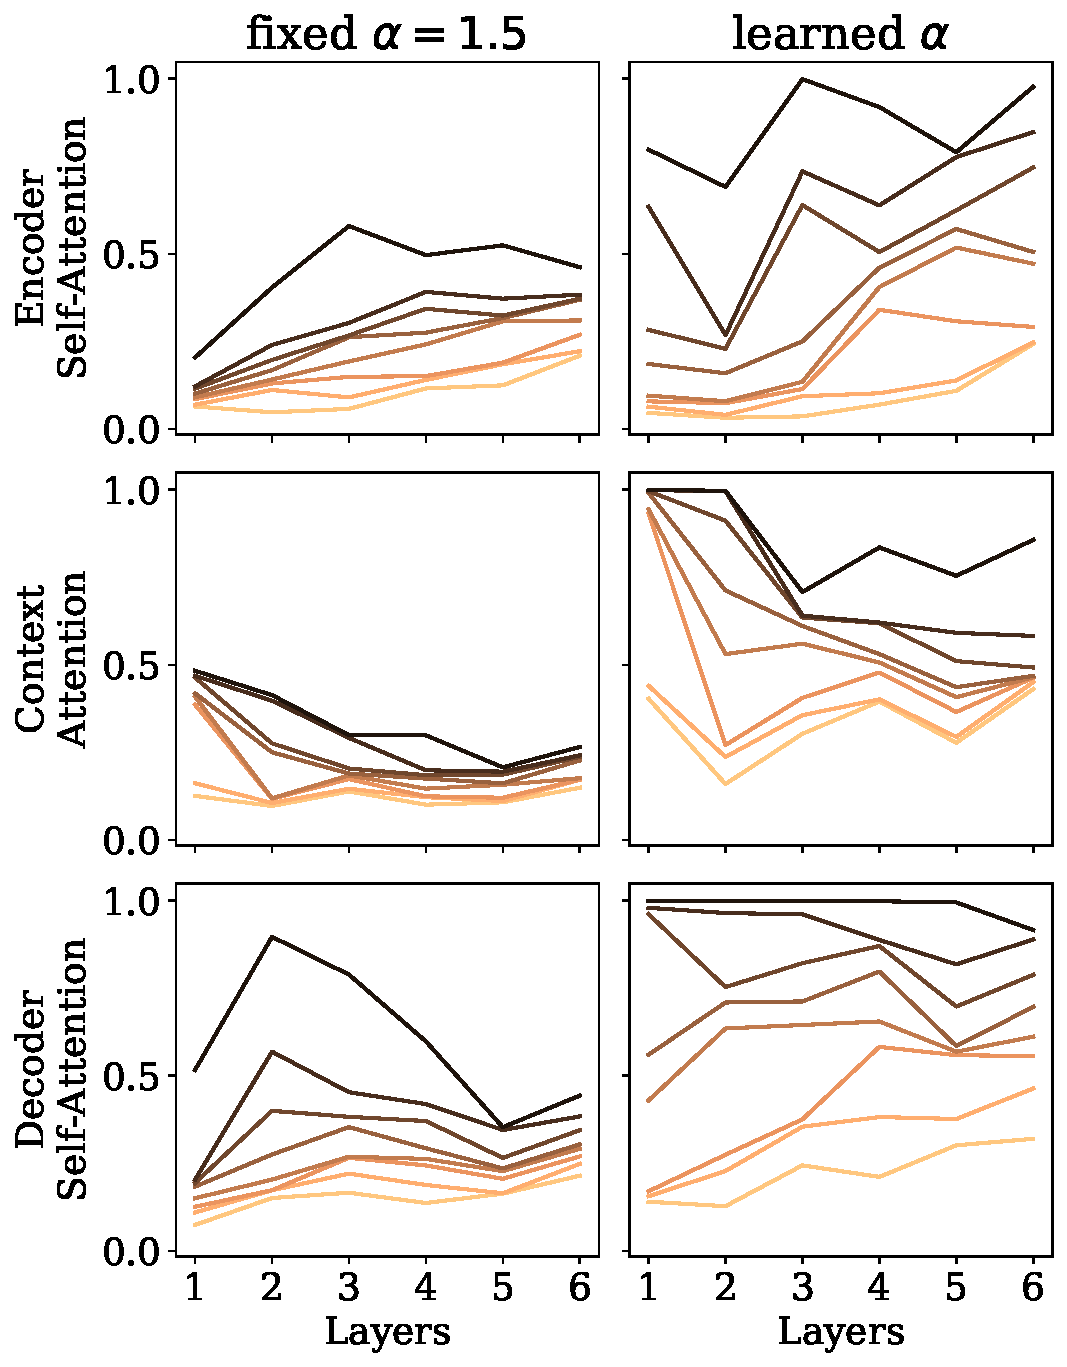
\includegraphics[width=\linewidth]{Figures/head_density_per_layer_ja.pdf}
        \caption{%
            \label{fig:head_density_per_layer_ja}%
            KFTT \langp{ja}{en}.}
    \end{subfigure}

    \begin{subfigure}[b]{.49\linewidth}
        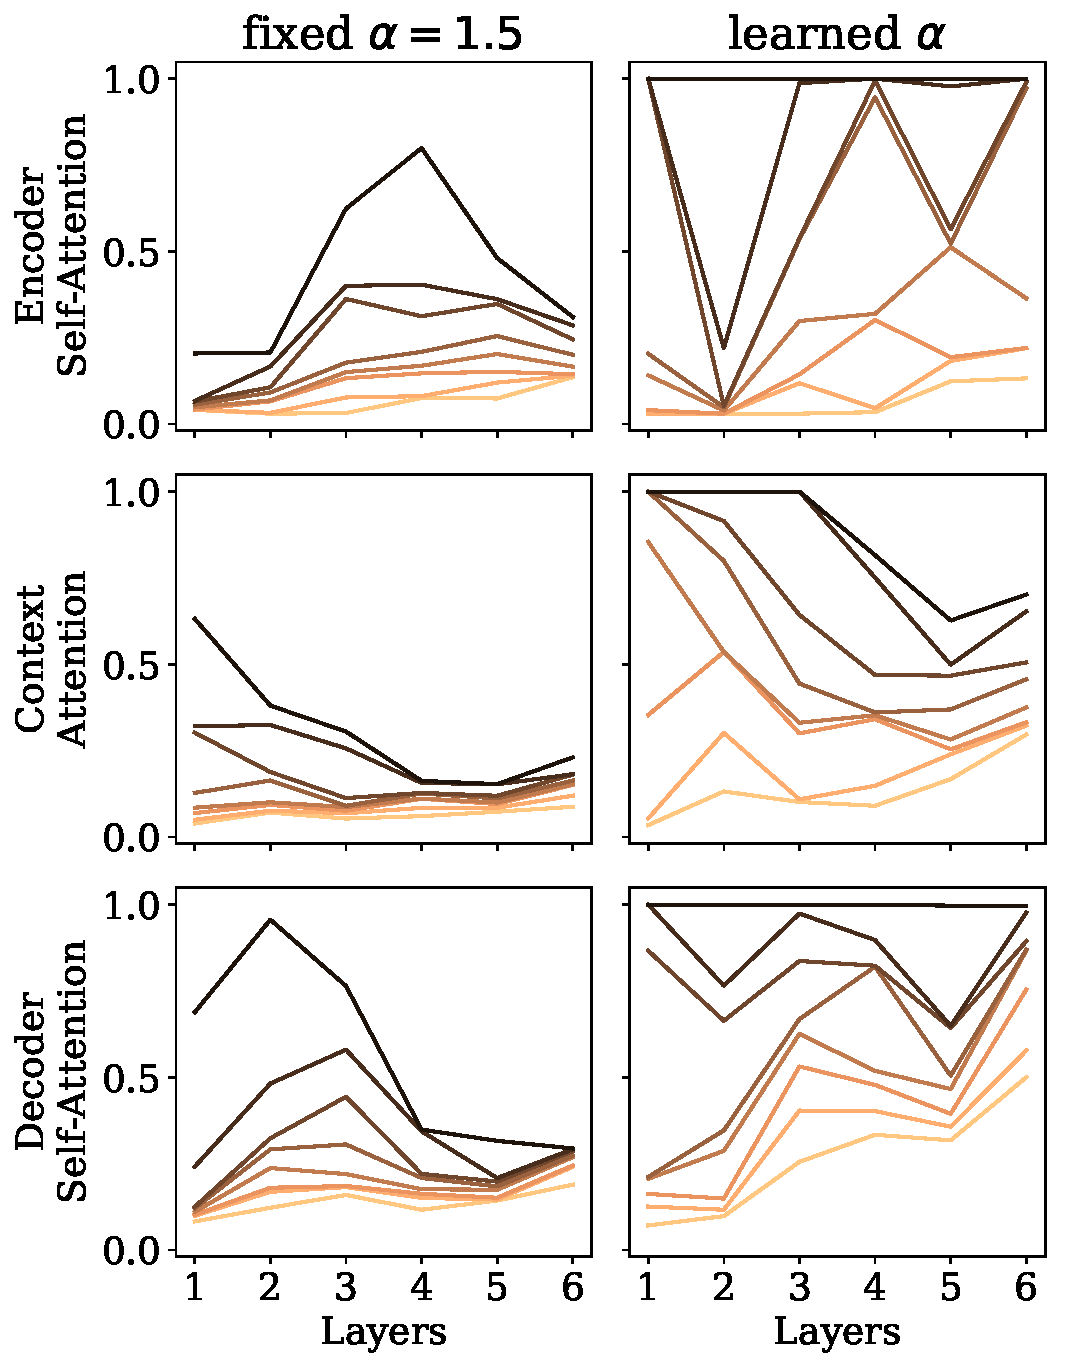
\includegraphics[width=\linewidth]{Figures/head_density_per_layer.pdf}
        \caption{%
            \label{fig:head_density_per_layer_en}%
            WMT 2014 \langp{en}{de}.}
    \end{subfigure}
    \begin{subfigure}[b]{.49\linewidth}
        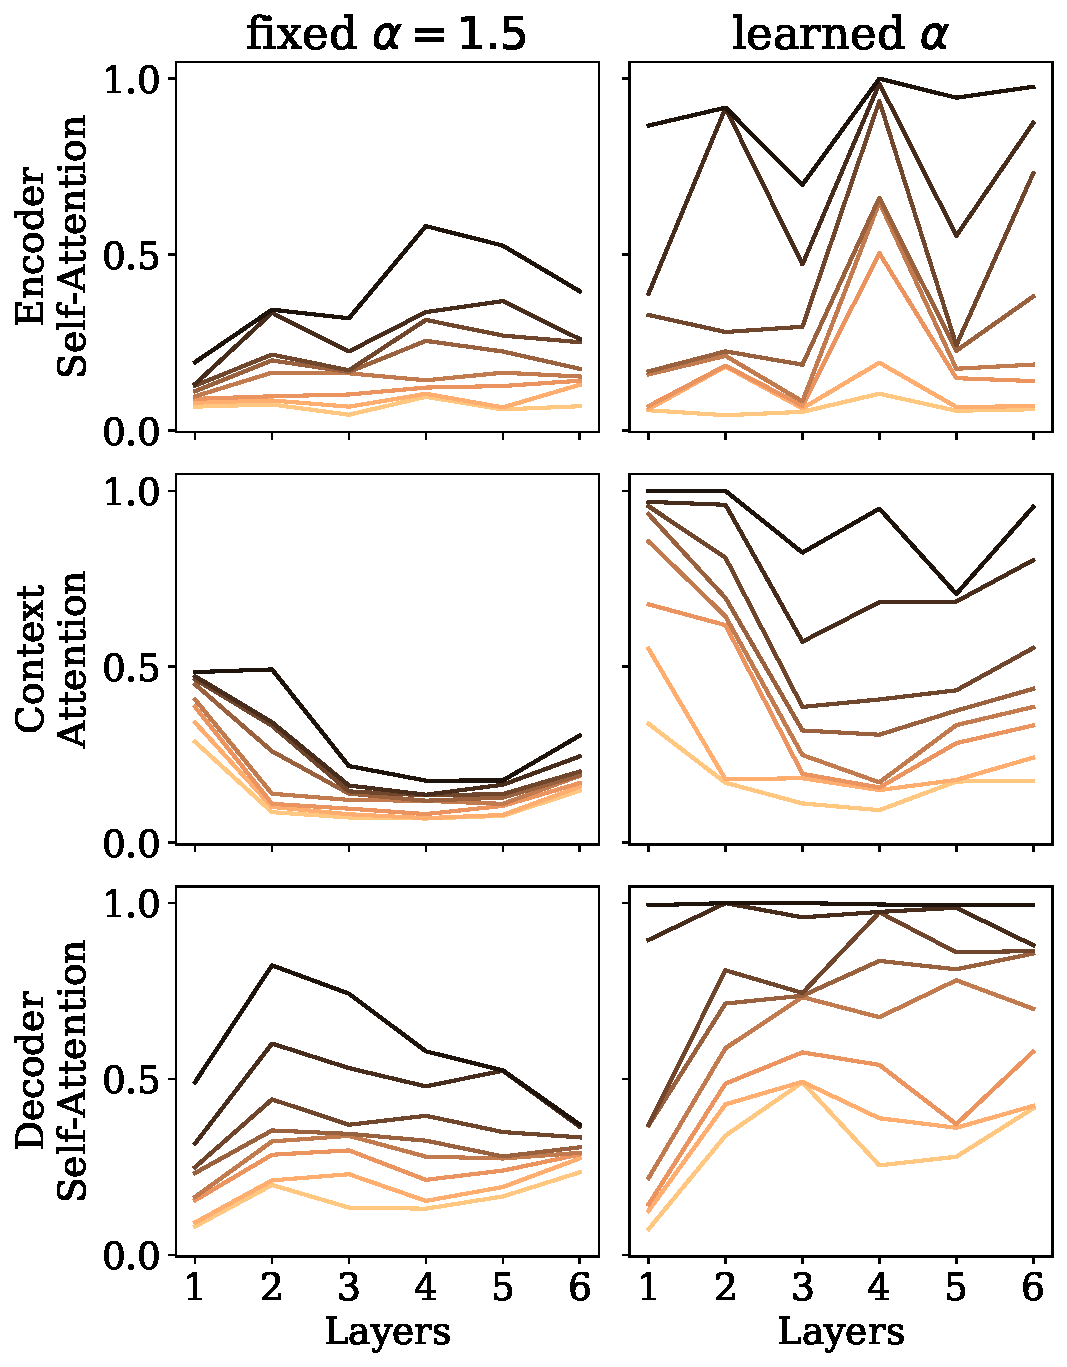
\includegraphics[width=\linewidth]{Figures/head_density_per_layer_de.pdf}
        \caption{%
            \label{fig:head_density_per_layer_de}%
            IWSLT 2017 \langp{de}{en}.}
    \end{subfigure}
    \caption{%
        \label{fig:head_density_per_layer}
        Head density per layer for fixed and learned $\alpha$. Each line
        corresponds to an attention head; lower values mean that that
        attention head is sparser. Learned $\alpha$ has higher variance.
    }
\end{figure}

\begin{figure}[!htbp]
    \centering
    \begin{subfigure}[b]{.49\linewidth}
        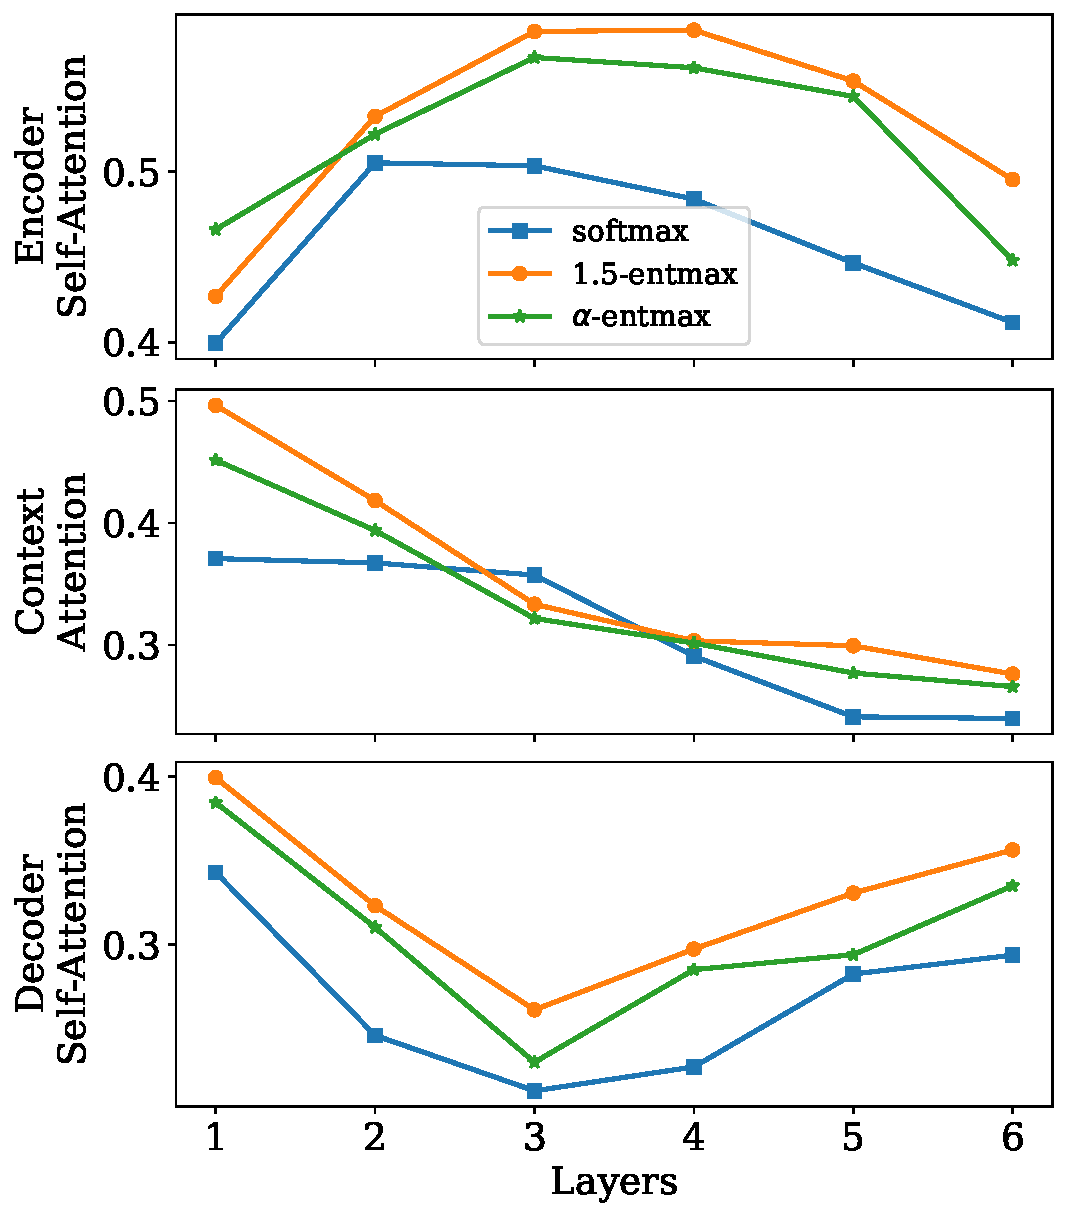
\includegraphics[width=\linewidth]{Figures/js_divs_ro.pdf}
        \caption{%
            \label{fig:js_divs_ro}%
            WMT 2016 \langp{ro}{en}.}
    \end{subfigure}
    \begin{subfigure}[b]{.49\linewidth}
        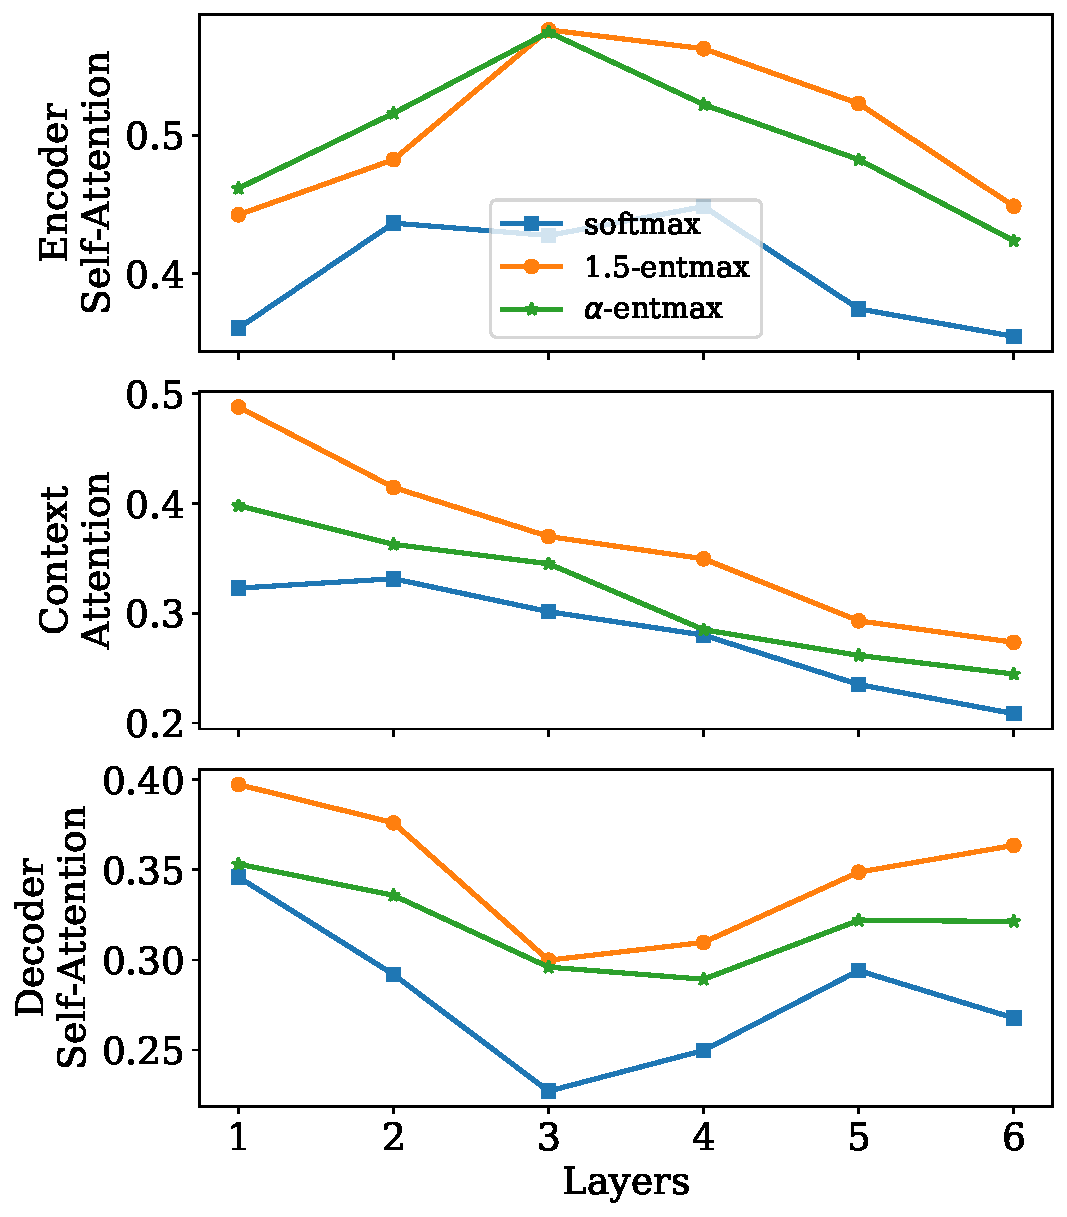
\includegraphics[width=\linewidth]{Figures/js_divs_ja.pdf}
        \caption{%
            \label{fig:js_divs_ja}%
            KFTT \langp{ja}{en}.}
    \end{subfigure}

    \begin{subfigure}[b]{.49\linewidth}
        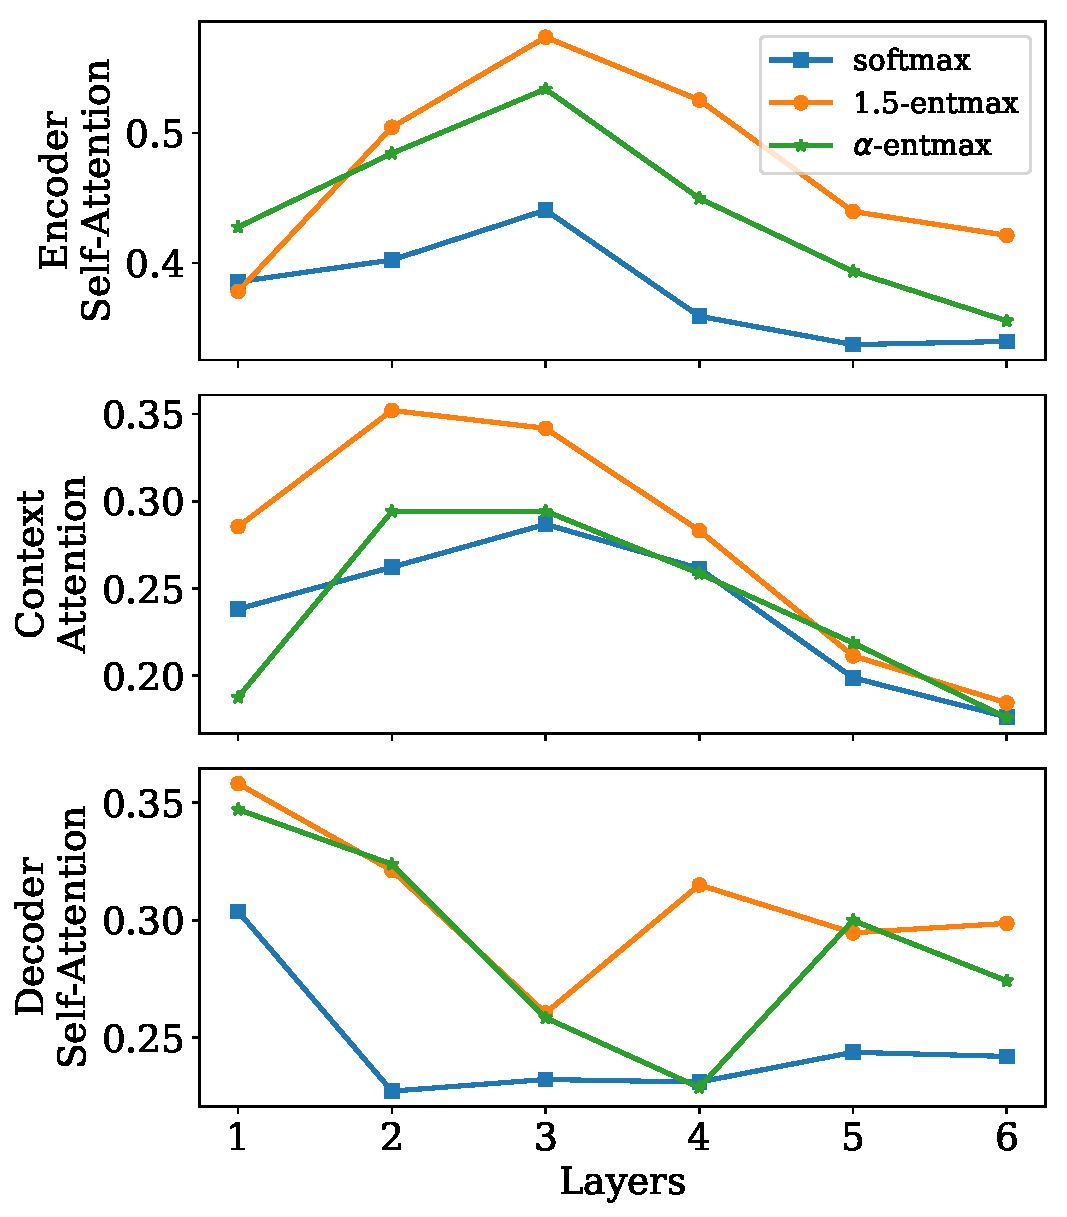
\includegraphics[width=\linewidth]{Figures/js_divs.pdf}
        \caption{%
            \label{fig:js_divs_en}%
            WMT 2014 \langp{en}{de}.}
    \end{subfigure}
    \begin{subfigure}[b]{.49\linewidth}
        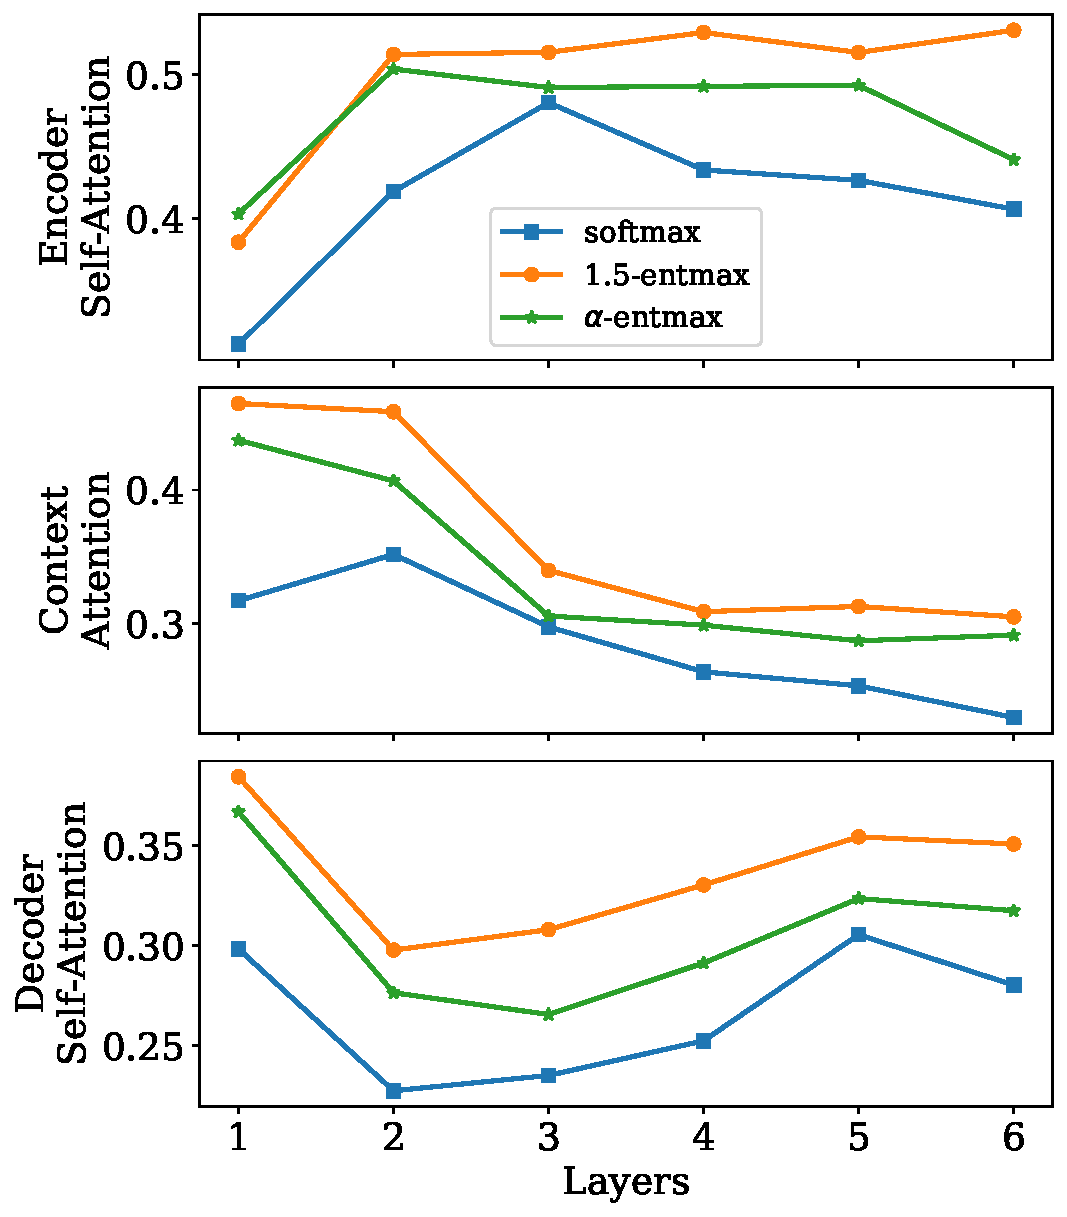
\includegraphics[width=\linewidth]{Figures/js_divs_de.pdf}
        \caption{%
            \label{fig:js_divs_de}%
            IWSLT 2017 \langp{de}{en}.}
    \end{subfigure}
    \caption{%
        \label{fig:js_divs}
        Jensen-Shannon Divergence between heads at each layer. Measures the
        disagreement between heads: the higher the value, the more the heads
        are disagreeing with each other in terms of where to attend. Models
        using sparse \entmaxtext have more diverse attention than the softmax
        baseline.
    }
\end{figure}

\paragraph*{Head diversity.} To measure the overall disagreement
between attention heads, as a measure of head diversity, we use the
following generalization of the Jensen-Shannon divergence:

\begin{equation}
    JS = \HHs\left(\frac{1}{H}\sum_{j=1}^H \bm{p}_{j}\right) -
    \frac{1}{H}\sum_{j=1}^{H}
    \HHs(\bm{p}_j)
\end{equation}

where $\bm{p}_j$ is the vector of attention weights assigned by head
$j$ to each word in the sequence, and $\HHs$ is the Shannon entropy,
base-adjusted based on the dimension of $\bm{p}$ such that $JS \leq
    1$. We average this measure over the entire validation set. The
higher this metric is, the more the heads are taking different roles
in the model.

\figref{fig:js_divs} shows that both sparse Transformer variants show
more diversity than the traditional softmax one. Interestingly,
diversity seems to peak in the middle layers of the encoder
self-attention and context attention, while this is not the case for
the decoder self-attention.

\begin{figure}[t]
    \centering
    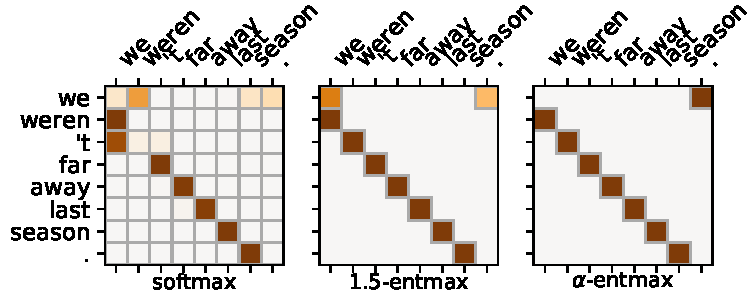
\includegraphics[width=0.95\columnwidth]{Figures/head_prev.pdf}
    \caption{
        Self-attention from the most confidently previous-position head in
        each model. The learned parameter in the $\alpha$-\entmaxtext model
        is $\alpha=1.91$. Quantitatively more confident, visual inspection
        confirms that the adaptive head behaves more consistently.}
    \label{fig:head_prev}
\end{figure}

\subsection{Identifying Head Specializations}\label{sec:spec}

Previous work pointed out some specific roles played by
different heads in the softmax Transformer
model~\citep{voita2018context,tang2018why,specialized}. Identifying
the specialization of a head can be done by observing the
type of tokens or sequences that the head often assigns most
of its attention weight; this is facilitated by sparsity.

\paragraph*{Positional heads.}
One particular type of head, as noted by \citet{specialized}, is the
positional head. These heads tend to focus their attention on either
the previous or next token in the sequence, thus obtaining
representations of the neighborhood of the current time step. In
\figref{fig:head_prev}, we show attention plots for such heads, found for
each of the studied models. The sparsity of our models allows these
heads to be more confident in their representations, by assigning the
whole probability distribution to a single token in the sequence.
Concretely, we may measure a positional head's \textbf{confidence} as
the average attention weight assigned to the previous token. The
softmax model has three heads for position $-1$, with median
confidence $93.5\%$. The $1.5$-\entmaxtext model also has three heads
for this position, with median confidence $94.4\%$. The adaptive
model has four heads, with median confidences $95.9\%$, the
lowest-confidence head being dense with $\alpha=1.18$, while the
highest-confidence head being sparse ($\alpha=1.91$).

For position $+1$, the models each dedicate one head, with confidence
around $95\%$, slightly higher for \entmaxtext. The adaptive model
sets $\alpha=1.96$ for this head.

\begin{figure}[t]
    \centering
    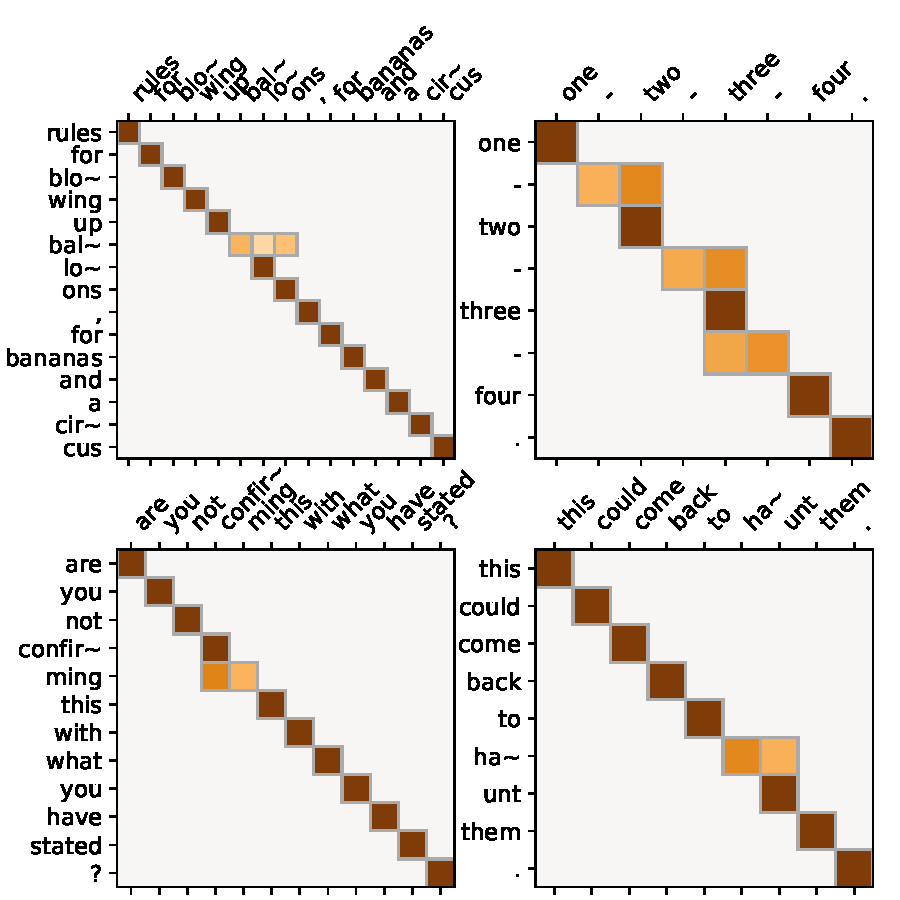
\includegraphics[width=0.95\columnwidth]{Figures/head_bpe}
    \caption{%layer 5+1 / head 6+1, alpha=1.33.
        BPE-merging head $(\alpha=1.91)$ discovered in the
        $\alpha$-\entmaxtext model. Found in the first encoder layer,
        this head learns to discover some subword units and combine their
        information, leaving most words intact. It places $99.09\%$ of
        its probability mass within the same BPE cluster as the current
        token: more than any head in any other model.}
    \label{fig:head_bpe}
\end{figure}

\begin{figure}[t]
    \centering
    \begin{subfigure}[b]{0.95\columnwidth}
        \centering
        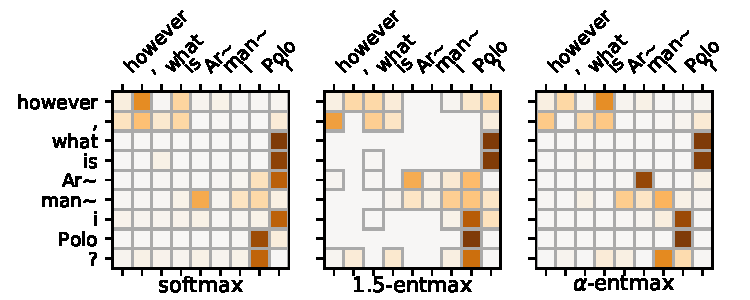
\includegraphics[width=\columnwidth]{Figures/head_interro.pdf}
    \end{subfigure}
    \begin{subfigure}[b]{0.95\columnwidth}
        \centering
        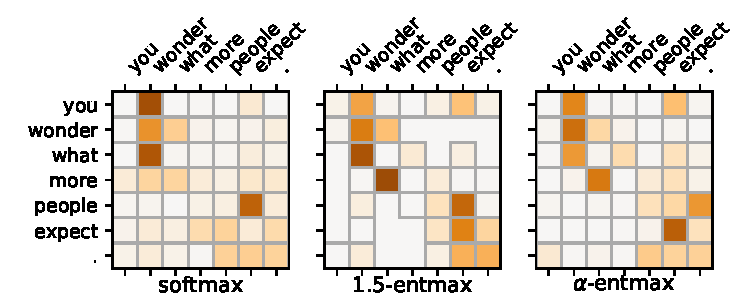
\includegraphics[width=\columnwidth]{Figures/head_interro_not.pdf}
    \end{subfigure}
    \caption{%layer 0+1 head 2+1 alpha=1.05
        Interrogation-detecting heads in the three models. The top sentence
        is interrogative while the bottom one is declarative but includes the
        interrogative word ``what''. In the top example, these {\it
                interrogation heads} assign a high probability to the question mark
        in the time step of the interrogative word (with $\geq 97.0\%$
        probability), while in the bottom example since there is no question
        mark, the same head does not assign a high probability to the last
        token in the sentence during the interrogative word time step.
        Surprisingly, this head prefers a low $\alpha=1.05$, as can be seen
        from the dense weights. This allows the head to identify the noun
        phrase ``Armani Polo" better.}
    \label{fig:head_interro}
\end{figure}

\begin{figure}[t]
    \centering
    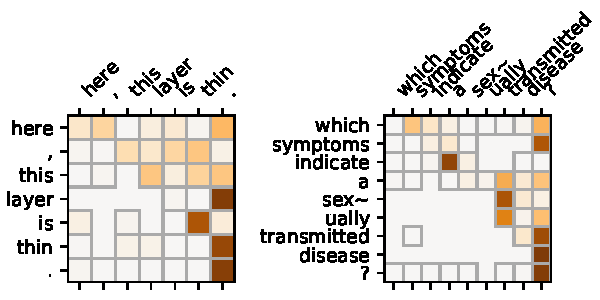
\includegraphics[
        width=0.95\columnwidth]{Figures/sparsity_difference.pdf}
    \caption{%layer 5+1 / head 6+1, alpha=1.33.
        Example of two sentences of similar length where the same head
        ($\alpha=1.33$) exhibits different sparsity. The longer phrase in the
        example on the right ``a sexually transmitted disease'' is handled
        with higher confidence, leading to more sparsity.
    }
    \label{fig:sparsity_difference}
\end{figure}

\paragraph*{BPE-merging head.}
Due to the sparsity of our models, we are able to identify other head
specializations, easily identifying which heads should be further analyzed.
In \figref{fig:head_bpe} we show one such head where the $\alpha$ value
is particularly high (in the encoder, layer 1, head 4 depicted in
\figref{fig:learning_alpha}). We found that this head most often looks at
the current time step with high confidence, making it a positional head
with offset $0$. However, this head often spreads weight sparsely
over 2-3 neighboring tokens, when the tokens are part of the same BPE
cluster\footnote{BPE-segmented words are denoted by $\sim$ in the
    Figures.} or hyphenated words. As this head is in the first layer, it
provides a useful service to the higher layers by combining
information evenly within some BPE clusters.

For each BPE cluster or cluster of hyphenated words,
we computed a score between 0 and 1 that corresponds to the
maximum attention mass assigned by any token to the rest of the
tokens inside the cluster in order to quantify the BPE-merging
capabilities of these heads.\footnote{If the
    cluster has size 1, the score is the weight the token assigns to
    itself.} There are not any attention heads in
the softmax model that are able to obtain a score over $80\%$, while
for $1.5$-\entmaxtext and $\alpha$-\entmaxtext there are two heads
in each ($83.3\%$ and $85.6\%$ for $1.5$-\entmaxtext and $88.5\%$ and
$89.8\%$ for $\alpha$-\entmaxtext).

\paragraph*{Interrogation head.}
On the other hand, in \figref{fig:head_interro} we show a head for which our
adaptively sparse model chose an $\alpha$ close to 1, making it
closer to softmax (also shown in {\it encoder, layer 1, head 3}
depicted in \figref{fig:learning_alpha}). We observe that this head
assigns a high probability to question marks at the end of the
sentence in time steps where the current token is interrogative, thus
making it an interrogation-detecting head. We also observe this type
of heads in the other models, which we also depict in
\figref{fig:head_interro}. The average attention weight placed on the
question mark when the current token is an interrogative word is
$98.5\%$ for softmax, $97.0\%$ for $1.5$-\entmaxtext, and $99.5\%$
for $\alpha$-\entmaxtext.

Furthermore, we can examine sentences where some tendentially sparse
heads become less so, thus identifying sources of ambiguity where the
head is less confident in its prediction. An example is shown in
\figref{fig:sparsity_difference} where sparsity in the same head differs
for sentences of similar length.

\section{Subsequent Work}\label{sec:subsequent_work_adapt}

\citet{correia2019adaptively} is, at the moment of writing, the most
influential work in this thesis. It is part of an early line of work
on Transformers that sparked interest in making this model more
efficient~\citep[\textit{inter
        alia}]{daras2020SMYRFEfficientAttention,
    li2020SACAcceleratingStructuring, merrill2021EffectsParameterNorm,
    roy2021EfficientContentBasedSparse}, using sparsity to allow for
Transformers to use longer contexts more
effectively~\citep[\textit{inter alia}]{jiang2020LongDocumentRanking,
    qiu2020BlockwiseSelfAttentionLong, sukhbaatar2021NotAllMemories}, and
being able to understand Transformers better~\citep[\textit{inter
        alia}]{you2020HardCodedGaussianAttention,
    rogers2020PrimerBERTologyWhat, pande2021headshypothesisunifying}.
This Transformer variant and $\alpha$-\entmaxtext have also proved
useful in medical applications~\citep{guo2020LearningLatentForests,
    yun2021SpecTrSpectralTransformer}.

Particularly connected to the present work,
\citet{treviso2021PredictingAttentionSparsity} tackles the quadratic
complexity that remains in our approach, as we had focused more on
the interpretability benefits of sparsity and not on its potential
computational benefits.
\citet{treviso2021PredictingAttentionSparsity} propose
\emph{Sparsefinder}, a method that predicts in advance the sparsity
pattern of $\alpha$-\entmaxtext, by projecting queries and keys into
a lower dimensional space, turning our approach into a
computationally efficient alternative to the original Transformer.

Still on the topic of computational efficiency,
\citet{ji2021DistributionSparsityInferencetime} focuses on inducing
sparsity on the attention heads only at inference time to avoid
unecessary training of new models and wasting of computational
resources. In order to achieve this, they propose a pruning and
quantization technique that does not lead to decreased performance.
To push the sparsity to the limit,
\citet{xu2021LearningHardRetrieval} propose a hard retrieval approach
that is able to make each attention mechanism attend to only a single
token. This approach also leads to similar performance to the
original Transformer but ends up having a 1.43 times faster decoding
performance in translation tasks.

Regarding the concept of Sparse Transformers,
\citet{yun2020ConnectionsareExpressive} unify several works that
sparsify Transformers in a single framework.
This unified framework is constructed through conditions based on the
sparsity pattern and the probability map. Once such conditions are
satisfied, the authors prove that some Sparse Transformers (of which
our approach is included) are universal approximators of any
continuous sequence-to-sequence function. Furthermore, they show that
when these Sparse Transformers have only $\mathcal{O}(n)$ connections (which is
in contrast to the constant $\mathcal{O}(n^2)$ connections of dense
Transformers), they still hold the same universal approximation
properties.

\citet{zhang2021SparseAttentionLinear} proposed another approach to
induce sparsity in each attention head of the Transformer. In this
work, instead of replacing the softmax with entmax, the authors
replace it with the ReLU activation. When compared to our approach,
Rectified Linear Attention (ReLA) obtains faster training and
decoding time, while achieving close performance in translation
tasks. In their analysis, they followed our methodology and found
that their method had higher JS Divergence than our own, suggesting
that attention heads using ReLA tend to be more diverse in where they
attend at each layer. Furthermore, ReLA is also able to assign null
attention for some queries, that is, to effectively deactivate an
attention head for a specific query, as it is able to assign zero
values to all tokens. Their analysis shows that the rate at which
null attention happens increases in deeper layers, which correlates
with our own analysis that deeper layers contain less information.
Moreover, \citet{zhang2021SparsifyingEncoderOutputs} achieves
sparsity by pruning entire sections of the encoder outputs in the
cross-attention of the decoder. This leads to a significant speed-up
during decoding. It drops whole sections from the source encodings to
speed up decoding, and the authors find that the tokens that end up
being dropped are often uninformative tokens, while the retained ones
are relatively rare.

On the topic of interpretability and understanding the inner workings
of Transformers, inspired by our analysis along with other
works~\citep{voita2019AnalyzingMultiHeadSelfAttention} that find that
encoder self-attention heads learn fixed patterns
(\secref{sec:spec}), \citet{raganato2020FixedEncoderSelfAttentiona}
fixes the attention pattern of all but one head in each layer,
letting only a single head in each layer learn its attention. Those
fixed patterns include the positional heads that focus on the
current, previous, and next token and the BPE-merging head that we
found. The parameter footprint of the model drastically decreases
thanks to these simplifications, and the authors show empirically
that translation quality does not drop significantly and even that,
in low-resource scenarios, this approach improves translation
performance.

\section{Final Remarks and Chapter Summary}

In the present chapter, we contributed with a novel strategy for
\textbf{learnable sparse} attention, and, in particular, for adaptively
sparse Transformers. We presented the first empirical analysis of
Transformers with sparse attention mappings (\ie, \entmaxtext),
showing potential in both translation accuracy as well as in model
interpretability and \textbf{transparency}.

In particular, we analyzed how the attention heads in the proposed
adaptively sparse Transformer can specialize more and with higher
confidence. Our adaptivity strategy relies only on gradient-based
optimization, side-stepping costly per-head hyper-parameter searches.
Given the impact of our work, we believe that approaches that
sparsify Transformers will continue to increase in the future, with
the objective of improving the architecture's efficiency and
transparency.

\cleardoublepage

\singlespacing